% ******************************* PhD Thesis Template **************************
% Please have a look at the README.md file for info on how to use the template

\documentclass[a4paper,12pt,fourier,numbered,print,oneside, PageStyleII]{Classes/PhDThesisPSnPDF}

% ******************************************************************************
% ******************************* Class Options ********************************
% *********************** See README for more details **************************
% ******************************************************************************

% `a4paper'(The University of Cambridge PhD thesis guidelines recommends a page
% size a4 - default option) or `a5paper': A5 Paper size is also allowed as per
% the Cambridge University Engineering Deparment guidelines for PhD thesis
%
% `11pt' or `12pt'(default): Font Size 10pt is NOT recommended by the University
% guidelines
%
% `oneside' or `twoside'(default): Printing double side (twoside) or single
% side.
%
% `print': Use `print' for print version with appropriate margins and page
% layout. Leaving the options field blank will activate Online version.
%
% `index': For index at the end of the thesis
%
% `draftclassic': For draft mode without loading any images (same as draft in book)
%
% `draft': Special draft mode with line numbers, images, and water mark with
% timestamp and custom text. Position of the text can also be modified.
%
% `abstract': To generate only the title page and abstract page with
% dissertation title and name, to submit to the Student Registry
%
% `chapter`: This option enables only the specified chapter and it's references
%  Useful for review and corrections.
%
% ************************* Custom Page Margins ********************************
%
% `custommargin`: Use `custommargin' in options to activate custom page margins,
% which can be defined in the preamble.tex. Custom margin will override
% print/online margin setup.
%
% *********************** Choosing the Fonts in Class Options ******************
%
% `times' : Times font with math support. (The Cambridge University guidelines
% recommend using times)
%
% `fourier': Utopia Font with Fourier Math font (Font has to be installed)
%            It's a free font.
%
% `customfont': Use `customfont' option in the document class and load the
% package in the preamble.tex
%
% default or leave empty: `Latin Modern' font will be loaded.
%
% ********************** Choosing the Bibliography style ***********************
%
% `authoryear': For author-year citation eg., Krishna (2013)
%
% `numbered': (Default Option) For numbered and sorted citation e.g., [1,5,2]
%
% `custombib': Define your own bibliography style in the `preamble.tex' file.
%              `\RequirePackage[square, sort, numbers, authoryear]{natbib}'.
%              This can be also used to load biblatex instead of natbib
%              (See Preamble)
%
% **************************** Choosing the Page Style *************************
%
% `default (leave empty)': For Page Numbers in Header (Left Even, Right Odd) and
% Chapter Name in Header (Right Even) and Section Name (Left Odd). Blank Footer.
%
% `PageStyleI': Chapter Name next & Page Number on Even Side (Left Even).
% Section Name & Page Number in Header on Odd Side (Right Odd). Footer is empty.
%
% `PageStyleII': Chapter Name on Even Side (Left Even) in Header. Section Number
% and Section Name in Header on Odd Side (Right Odd). Page numbering in footer

% ********************************** Preamble **********************************
% Preamble: Contains packages and user-defined commands and settings
% ******************************************************************************
% ****************************** Custom Margin *********************************

% Add `custommargin' in the document class options to use this section
% Set {innerside margin / outerside margin / topmargin / bottom margin}  and
% other page dimensions
\ifsetCustomMargin
  \RequirePackage[left=37mm,right=30mm,top=35mm,bottom=30mm]{geometry}
  \setFancyHdr % To apply fancy header after geometry package is loaded
\fi

% Add spaces between paragraphs
%\setlength{\parskip}{0.5em}
% Ragged bottom avoids extra whitespaces between paragraphs
\raggedbottom
% To remove the excess top spacing for enumeration, list and description
%\usepackage{enumitem}
%\setlist[enumerate,itemize,description]{topsep=0em}

% *****************************************************************************
% ******************* Fonts (like different typewriter fonts etc.)*************

% Add `customfont' in the document class option to use this section

\ifsetCustomFont
  % Set your custom font here and use `customfont' in options. Leave empty to
  % load computer modern font (default LaTeX font).
  %\RequirePackage{helvet}

  % For use with XeLaTeX
  %  \setmainfont[
  %    Path              = ./libertine/opentype/,
  %    Extension         = .otf,
  %    UprightFont = LinLibertine_R,
  %    BoldFont = LinLibertine_RZ, % Linux Libertine O Regular Semibold
  %    ItalicFont = LinLibertine_RI,
  %    BoldItalicFont = LinLibertine_RZI, % Linux Libertine O Regular Semibold Italic
  %  ]
  %  {libertine}
  %  % load font from system font
  %  \newfontfamily\libertinesystemfont{Linux Libertine O}
\fi

% *****************************************************************************
% **************************** Custom Packages ********************************

% ************************* Algorithms and Pseudocode **************************

%\usepackage{algpseudocode}


% ********************Captions and Hyperreferencing / URL **********************

% Captions: This makes captions of figures use a boldfaced small font.
%\RequirePackage[small,bf]{caption}

\RequirePackage[labelsep=space,tableposition=top]{caption}
\renewcommand{\figurename}{Fig.} %to support older versions of captions.sty


% *************************** Graphics and figures *****************************

%\usepackage{rotating}
%\usepackage{wrapfig}

% Uncomment the following two lines to force Latex to place the figure.
% Use [H] when including graphics. Note 'H' instead of 'h'
%\usepackage{float}
%\restylefloat{figure}

% Subcaption package is also available in the sty folder you can use that by
% uncommenting the following line
% This is for people stuck with older versions of texlive
%\usepackage{sty/caption/subcaption}
\usepackage{subcaption}

% ********************************** Tables ************************************
\usepackage{booktabs} % For professional looking tables
\usepackage{multirow}

%\usepackage{multicol}
%\usepackage{longtable}
%\usepackage{tabularx}


% *********************************** SI Units *********************************
\usepackage{siunitx} % use this package module for SI units


% ******************************* Line Spacing *********************************

% Choose linespacing as appropriate. Default is one-half line spacing as per the
% University guidelines

% \doublespacing
% \onehalfspacing
% \singlespacing


% ************************ Formatting / Footnote *******************************

% Don't break enumeration (etc.) across pages in an ugly manner (default 10000)
%\clubpenalty=500
%\widowpenalty=500

%\usepackage[perpage]{footmisc} %Range of footnote options


% *****************************************************************************
% *************************** Bibliography  and References ********************

%\usepackage{cleveref} %Referencing without need to explicitly state fig /table

% Add `custombib' in the document class option to use this section
\ifuseCustomBib
   \RequirePackage[square, sort, numbers, authoryear]{natbib} % CustomBib

% If you would like to use biblatex for your reference management, as opposed to the default `natbibpackage` pass the option `custombib` in the document class. Comment out the previous line to make sure you don't load the natbib package. Uncomment the following lines and specify the location of references.bib file

%\RequirePackage[backend=biber, style=numeric-comp, citestyle=numeric, sorting=nty, natbib=true]{biblatex}
%\bibliography{References/references} %Location of references.bib only for biblatex

\fi

% changes the default name `Bibliography` -> `References'
\renewcommand{\bibname}{References}


% ******************************** Roman Pages *********************************
% The romanpages environment set the page numbering to lowercase roman one
% for the contents and figures lists. It also resets
% page-numbering for the remainder of the dissertation (arabic, starting at 1).

\newenvironment{romanpages}{
  \setcounter{page}{1}
  \renewcommand{\thepage}{\roman{page}}}
{\newpage\renewcommand{\thepage}{\arabic{page}}}


% ******************************************************************************
% ************************* User Defined Commands ******************************
% ******************************************************************************

% *********** To change the name of Table of Contents / LOF and LOT ************

%\renewcommand{\contentsname}{My Table of Contents}
%\renewcommand{\listfigurename}{My List of Figures}
%\renewcommand{\listtablename}{My List of Tables}


% ********************** TOC depth and numbering depth *************************

\setcounter{secnumdepth}{2}
\setcounter{tocdepth}{2}


% ******************************* Nomenclature *********************************

% To change the name of the Nomenclature section, uncomment the following line

\renewcommand{\nomname}{Glossar}


% ********************************* Appendix ***********************************

% The default value of both \appendixtocname and \appendixpagename is `Appendices'. These names can all be changed via:

%\renewcommand{\appendixtocname}{List of appendices}
%\renewcommand{\appendixname}{Appndx}

% *********************** Configure Draft Mode **********************************

% Uncomment to disable figures in `draftmode'
%\setkeys{Gin}{draft=true}  % set draft to false to enable figures in `draft'

% These options are active only during the draft mode
% Default text is "Draft"
%\SetDraftText{DRAFT}

% Default Watermark location is top. Location (top/bottom)
%\SetDraftWMPosition{bottom}

% Draft Version - default is v1.0
%\SetDraftVersion{v1.1}

% Draft Text grayscale value (should be between 0-black and 1-white)
% Default value is 0.75
%\SetDraftGrayScale{0.8}


% ******************************** Todo Notes **********************************
%% Uncomment the following lines to have todonotes.

%\ifsetDraft
%	\usepackage[colorinlistoftodos]{todonotes}
%	\newcommand{\mynote}[1]{\todo[author=kks32,size=\small,inline,color=green!40]{#1}}
%\else
%	\newcommand{\mynote}[1]{}
%	\newcommand{\listoftodos}{}
%\fi

% Example todo: \mynote{Hey! I have a note}



\usepackage{extsizes}
\usepackage[ngerman]{babel}
\usepackage{enumerate}					%For enumeration counter
\usepackage{footnote}					%For footnotes

%\usepackage{draftwatermark}				%Sets watermarks up.
%\SetWatermarkScale{0.3}
%\SetWatermarkText{\bf Draft: \today}

\setlength{\parfillskip}{0pt plus 1fil}  % fix last line of a paragraph



% ************************ Thesis Information & Meta-data **********************
% Thesis title and author information, refernce file for biblatex
% ************************ Thesis Information & Meta-data **********************
%% The title of the thesis
\title{Kritische Erfolgsfaktoren für ein Computer Emergency Response Team (CERT)}
%\texorpdfstring is used for PDF metadata. Usage:
%\texorpdfstring{LaTeX_Version}{PDF Version (non-latex)} eg.,
%\texorpdfstring{$sigma$}{sigma}

%% The full name of the author
\author{Michael Kohler}

%% Department (eg. Department of Engineering, Maths, Physics)
\dept{Bachelor of Science in Computer Science}

%% University and Crest
\university{Fernfachhochschule Schweiz}
% Crest minimum should be 30mm.
\crest{
\includegraphics[width=0.5\textwidth]{ffhs}}

%% Supervisor (optional)
%\supervisor{Prof. Kenichi Soga}
%% Supervisor Role (optional) - Supervisor (default) or advisor
%\supervisorrole{Advisor: }

%% Advisor (optional)
%\advisor{Prof. Malcolm Bolton}
%% Advisor Role (optional) - Advisor (default) or leave empty
%\advisorrole{Advisor: }


%% You can redefine the submission text:
% Default as per the University guidelines:
% ``This dissertation is submitted for the degree of''
\renewcommand{\submissiontext}{Diese Arbeit ist Teil des Moduls}

%% Full title of the Degree
\degreetitle{SEMA}

%% Submission date
% Default is set as {\monthname[\the\month]\space\the\year}
%\degreedate{September 2014} 

%% Meta information
\subject{LaTeX} \keywords{{LaTeX} {SEMA} {Computer Science} {Fernfachhochschule Schweiz}}

% ***************************** Abstract Separate ******************************
% To printout only the titlepage and the abstract with the PhD title and the
% author name for submission to the Student Registry, use the `abstract' option in
% the document class.

\ifdefineAbstract
 \pagestyle{empty}
 \includeonly{Abstract/abstract}
\fi

% ***************************** Chapter Mode ***********************************
% The chapter mode allows user to only print particular chapters with references
% Title, Contents, Frontmatter are disabled by default
% Useful option to review a particular chapter or to send it to supervisior.
% To use choose `chapter' option in the document class

\ifdefineChapter
 \includeonly{Chapters/chapter3}
\fi

% ******************************** Front Matter ********************************
\begin{document}

\frontmatter

\begin{titlepage}
  \maketitle
\end{titlepage}

% ************************** Thesis Abstract *****************************
% Use `abstract' as an option in the document class to print only the titlepage and the abstract.
\begin{abstract}
Aufgabenstellung gemäss Dozenten-Themenliste des Moduls SEMA:\linebreak
\begin{quote}
``Ein Computer-Notfallteam oder auch Computer Emergency Response Team (CERT) trägt mit seiner Expertise zum Thema IT-Sicherheit massgeblich dazu bei, dass möglichen Angriffen auf IT-Infrastrukturen bereits im Vorfeld wirksam begegnet werden kann. Auch nach einem IT-Sicherheitsvorfall ist ein CERT bei der Wiederaufnahme des Regelbetriebs und der Ermittlung der Verursacher eine nahezu unverzichtbare Unterstützung. Diese Arbeit erläutert zunächst die notwendigen Grundlagen zum Verständnis eines CERTs undefasst sich danach intensiv mit der Fragestellung, anhand welcher Faktoren der Erfolg eines Computer- Notfallteams festgemacht werden kann und welche Punkte sowohl bei dessen Aufbau als auch dessen Betrieb beachtet werden sollten.``
\end{quote}
\end{abstract}


% *********************** Adding TOC and List of Figures ***********************

\tableofcontents

\listoffigures

% \printnomenclature[space] space can be set as 2em between symbol and description
%\printnomenclature[3em]

\printnomenclature

% ******************************** Main Matter *********************************
\mainmatter

\setcounter{page}{1}
\pagenumbering{arabic}
%*******************************************************************************
%*********************************** First Chapter *****************************
%*******************************************************************************

\chapter{Grundlagen}  %Title of the First Chapter

\ifpdf
    \graphicspath{{Figs/Raster/}{Figs/PDF/}{Figs/}}
\else
    \graphicspath{{Figs/Vector/}{Figs/}}
\fi


%********************************** %First Section  **************************************

\section{Definition}
Ein Computer Emergency Response Team (CERT) (Deutsch: ```Computer-Notfall-Team```) ist ein Team, welches sich um IT-Sicherheit kümmert. Es analysiert mögliche Bedrohungen und wirkt möglichen Angriffen und Bedrohungen bereits vor dem Eintreten entgegen. Sollte es trotzdem zu einem Angriff kommen, ist das CERT verantwortlich die Ursachen zu ermitteln, dagegen vorzugehen und unterstützt bei der Wiederaufnahme des Regelbetriebs massgeblich mit.

\section{CERT und CSIRT}
\paragraph{CERT}Der Begriff ``CERT`` wurde vom Software Engineering Institute an der Carnegie Mellon University geprägt. Die CERT Devision arbeitet u.a. an der Forschung von Cybersecurity-Themen. Der Fokus liegt hierbei jedoch nicht nur auf der Forschung, sondern auch an der Entwicklung von Informationen zu IT-Sicherheitsthemen. Zusätzlich arbeitet die Devision auch mit Softwareherstellern, um die Sicherheit von Softwareprodukten zu erhöhen.~\citep{cert} Die CERT Devision wurde im Jahre 1988 nach dem Auftreten des Morris-Wurms an der Carnegie Mellon University in Pittsburg, Pensylvania in den USA gegründet.~\citep{homonym} Finanziert wurde diese Gründung durch das amerikanische Department of Defense. In den USA ist der Begriff ```CERT``` markenrechtlich geschützt und gehört der Carnegie Mellon University.
\paragraph{CSIRT}Aus diesem Grund werden CERT auch häufig als Computer Security Incident Responsive Team (CSIRT) bezeichnet. Es gibt jedoch auch einige Ausnahmen, wie z.B. der CERT-Bund des deutschen Bundesamtes für Sicherheit in der Informationstechnik. \\
\\
In dieser Arbeit werde ich beide Begriffe verwenden, wobei ich CERT als Markenname und CSIRT als Konzeptbegriff verwende.

\section{Grundlegende Aufgaben}
Durch das schnelle Wachstum und die Popularität des Internets befinden sich viele Firmen sehr schnell im Visier von Cyberattacken. Fast alle Firmen haben schützenswerte Informationen in ihren Systemen, welche deshalb genügend geschützt werden müssen. Bedrohungen sind nicht zwingend nur E-Spionage oder Konkurrenz. Bedrohungen durch das Internet reichen von ``normalen`` Viren und Ransomware~\citep{ransomware} bis zum gezielten Eindringen in Computernetzwerke von Firmen, um Daten zu entwenden oder zerstören. Eine komplette Abschottung und Eliminierung aller Angriffsvektoren ist Utopie, daher muss hierfür ein Mittelweg gefunden werden. \\
\\
Um diese Grundlage als CSIRT zu erfüllen, gehören folgende Aufgabenbereiche zum Tätigkeitsbereich eines CSIRTs:

\begin{itemize}
\item Analyse der Bedrohungslage
\item Erkennung von Angriffen im Voraus
\item Erkennung von momentanen Angriffen
\item Elimierung von momentanen Angriffen
\item Erarbeitung eines Notfallkonzeptes
\item Sofortiges Eingreifen in einer Bedrohungslage und direkte Massnahmen zur Sicherung und Notfall-Betriebes von kritischen Geschäftsprozessen
\item Unterstützung bei der Wiederaufnahme des Regelbetriebs
\item Koordination mit anderen CSIRTs
\end{itemize}

\section{Forum of Incident Response and Security Teams}
Nachdem 1988 das erste CERT an der Cornegie Mellon University gegründet wurde, gründete sich 1990 der Dachverband ``Forum of Incident Response and Security Teams``. \\
\\
Die FIRST fördert die globale Zusammenarbeit zwischen Notfallteams und definiert ``Best Practices``. Zudem werden Frameworks durch die FIRST zur Verfügung gestellt, welche den Aufbau und Betrieb von CERTs definieren, sowie auch Weiterbildungsmaterial um die globale Akzeptanz und das Wissen zu Security Incident Management zu fördern.

\section{CERT in der Schweiz}
Das bekannteste CERT in der Schweiz wird von SWITCH Information Technology Services gestellt. SWITCH ist verantwortlich für die .ch und .li Domains. Zusätzlich erbringt SWITCH auch Dienstleistungen im nationalen Forschung- und Bildungsnetzwerk und verlinkt Schweizer Universitäten mit anderen, internationalen Universitäten.\\
\\
Dank des CERTs der SWITCH ist die Schweizer Top Level Domain (TLD) eine der sichersten der Welt und die sicherste TLD Europas. ~\citep{switch}

\subsection{Gründung des SWITCH CERT}
Die CERT-Abteilung von SWITCH existiert bereits seit 20 Jahren. 1994 wird der Aufbau einer Fachstelle für Sicherheitsfragen geschaffen. Gemäss Geschäftsbericht der SWITCH dieses Jahres werden bereits einige sicherheitsrelevante Anfragen von Kunden der SWITCH beantwortet und die SWITCH informierte über bekanntgewordene Sicherheitsverletzungen. Die Akkreditierung der SWITCH-CERT erfolgt 1996 durch das CERT/CC der CERT-Koordinationsstelle der Carnegie Mellon University.

\section{CERT in Deutschland}
Auch in Deutschland sind mehrere CERTs tätig. Neben dem CERT der Universität Stuttgart sowie dem CERT des deutschen Forschungsnetzwerkes hatte sich auch Mcert etabliert. Das Mcert richtete sich vorallem an kleine und mittlere Unternehmen. Mittlerweile existiert die Mcert nicht mehr und wird durch das neu erschaffene CERT-Bund weitergeführt.

\subsection{CERT-Bund}

CERT-Bund ist die CERT des  Bundesamts für Sicherheit in der Informationstechnik (BSI). \\
\\
``CERT-Bund hat das Ziel als zentrale Anlaufstelle für präventive und reaktive Maßnahmen mit Bezug auf sicherheits- und verfügbarkeitsrelevante Vorfälle in Computersystemen zu fungieren. IT-Sicherheitsvorfälle werden in Zusammenarbeit mit Betroffenen von CERT-Bund bearbeitet.``~\citep{certbund} \\
\\
Das CERT-Bund bietet unter anderem folgende Dienstleistungen an: 24-Stunden-Support, Betrieb eines Lagezentrums, Analyze von und Empfehlungen zu Vorfällen anhand von Meldungen, Warndienste, Alarmierung der Bundesverwaltung

\subsection{Bürger-CERT}
Da das CERT-Bund nicht alle Anliegen von Privaten bearbeiten kann, wurde eine separate CERT ins Leben gerufen. Dieses Projekt untersteht auch dem deutschen BSI. Privatpersonen sowie Unternehmen können sich kostenlos diverse Dienstleistungen wie z.B. Gefährdungsnewsletter und -Alarmierungen via E-Mail abonnieren. So können sich auch kleinere Unternehmen über die Gefahrenlage informieren und proaktiv nach der Alarmierung gegen Gefahren schützen.

\section{Security Incident Management}
Security Incident Management bezeichnet das Vorgehen, wie bei Bedrohungen der IT-Sicherheit vorgegangen werden muss. Dies involviert Monitoring und Erkennen von Bedrohungen in Computer oder Computer-Netzwerken. Tritt ein Incident (Event) ein, wird dieses gemäss definiertem Prozess effektiv behandelt. Wie ein solcher Prozess aussehen kann, wird später veranschaulicht. \\
\\
Security Incident Management ist die Grundlage für CISRT. Ohne Definition, wie mit Security Incidents umgegangen werden soll, kann das Response Team nicht arbeiten. Security Incident Management ist eines der wichtigsten Teilgebiete der IT-Security und dadurch Teil der ISO-27000 Familie. ISO-27035~\citep{iso27035} definiert die Grundlagen für das Security Incident Management und definiert fünf Phasen.

\subsection{Phase 1: Prepare}
In der Vorbereitungsphase ist das Ziel ein CSIRT aufzubauen und die dafür benötigten Prozessgrundlagen zu erarbeiten. Sobald diese Prozesse und das Team definiert sind, kann mit dem Monitoring von Bedrohungen und Identifizieren von Incidents fortgeführt werden. \\
\\
Wichtige Fragen:
\begin{itemize}
\item Wie soll auf ein Incident reagiert werden?
\item Wer reagiert wie und wann?
\item Wie ist der Eskalationsprozess aufgebaut?
\item Wie setzt sich das Response Team zusammen?
\item Wer wird wann informiert?
\item Wo werden Incidents dokumentiert?
\item Wie werden Incidents in Zukunft vermieden?
\end{itemize}

\subsection{Phase 2: Identify}
In der Identifikationsphase geht es darum, dass Bedrohungen und Incidents schnell und korrekt identifiziert werden können. Sobald ein Incident identifiziert wird, muss dieser sofort gemäss Prozessdefinition gemeldet werden. Je nach Prozess kann dies in verschiedenen Tools gemeldet werden. Ein Beispiel dafür wäre ein Ticket beim Service Desk. Hierbei ist es wichtig, dass die korrekte Prioriät übernommen wird und nicht innerhalb der anderen Tickets untergeht.\\
\\
Der ISO-27035-Standard definiert Vorlagen für das Reporting von Security Incidents. Diese dürfen entsprechend verwendet werden und können, falls nötig, auch an die eigene Unternehmensstruktur angepasst werden.

\subsection{Phase 3: Assess}
In der Assess-Phase wird ermittelt, wie mit diesem Incident vorgangen werden kann.\\
\\
Fragen, die sich das CSIRT stellen muss in dieser Phase beinhalten unter anderem:

\begin{itemize}
\item Muss das System offline genommen werden bis der Incident behoben ist?
\item Müssen forensische Daten gesammelt werden, bevor das System wieder funktionstüchtig gemacht werden kann?
\item Reicht es aus, das System zu patchen und wieder online zu bringen?
\item Muss das System komplett neu aufgesetzt werden?
\end{itemize}

\subsection{Phase 4: Respond}
Sind die möglichen Optionen klar und die beste(n) davon gewählt, muss der Incident behoben werden. Die definierten Aktionen werden durchgeführt bis das System wieder im Normalbetrieb ist. Ist dies erledigt, kann der Incident geschlossen werden.

\subsection{Phase 5: Learn}
Der Incident ist zwar gelöst, aber der Prozess ist noch nicht fertig angewendet. Phase 5 definiert ``Lessions learnt``. Um in der Zukunft besser und effektiver auf einen Incident zu reagieren, werden die durch diesen Incident gewonnenen Erkenntnisse analysiert und dokumentiert. Nur so kann sichergestellt werden, dass sich das CSIRT mit den Erkenntnissen auseinandersetzt und diese dazu verwendet, den Prozess zu optimieren. Da ein Prozess nie perfekt ist, sollten diese Erkenntnisse in die Prozessoptimierung einfliessen. Dabei ist es wichtig, dass dies regelmässig gemacht wird, damit der Prozess immer möglichst effektiv und effizient abgearbeitet werden kann.

\begin{figure}
  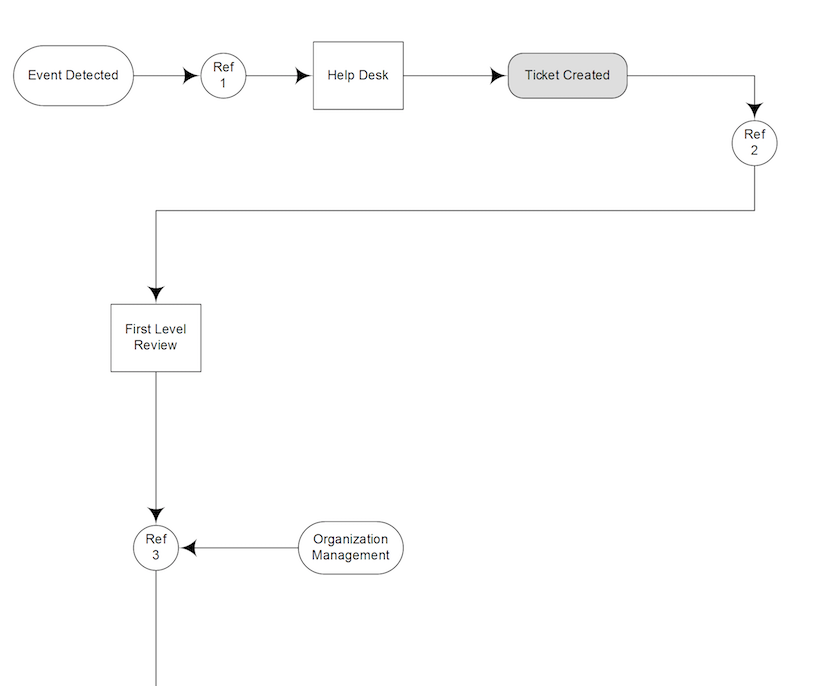
\includegraphics[width=\textwidth]{SIMExample}
    \caption{Auszug aus einem Security Incident Management Workflow. Image: CC-BY 2.5, Autor: Michael Berman}
    \label{fig:SIMExample}          
\end{figure}

\nomenclature[z-cert]{$CERT$}{Computer Emergency Response Team}
\nomenclature[z-csirt]{$CSIRT$}{Computer Security Incident Response Team}
\nomenclature[z-tld]{$TLD$}{Top Level Domain}

%*******************************************************************************
%****************************** Second Chapter *********************************
%*******************************************************************************

\chapter{Aufbau und Betrieb eines CERT}

\ifpdf
    \graphicspath{{Figs/Raster/}{Figs/PDF/}{Figs/}}
\else
    \graphicspath{{Figs/Vector/}{Figs/}}
\fi

\section{Aufbau}
Da die Effizienz ein Grundbaustein eines CERT ist, muss bereits der Aufbau vorsichtig geplant werden. Dieser Teil der Arbeit orientiert sich am "CSIRT Setting up Guide" der ENISA.~\citep{enisaguide} \\
\\
Die ENISA ist die European Union Agency for Network and Information Security. Die Aufgabe der ENISA ist es, die erforderliche hochgradige Netz- und Informationssicherheit in der EU zu gewährleisten. Dafür berät sie die Behörden der EU-Staaten sowie EU-Institutionen zur Netz- und Informationssicherheit. Zudem dient sie als Forum für den Austausch bewährter Verfahren sowie als Kontakt zwischen EU-Institutionen, Behörden und Unternehmen.

\subsection{Analyse der Klientel}
Bevor der Geschäftsplan ausgearbeitet werden kann, müssen die Anforderungen der Kunden (``Klientel`` hat sich im CERT-Umfeld als Ausdruck dafür etabliert) genau analysiert werden. Da CERT in verschiedenen Szenarien eingesetzt werden können, ist dies ein wichtiger Schritt. Auch das Umfeld des Klientels hat eine grosse Auswirkung auf die Planung des CERTs sowie auf dessen Betriebsmodus. \\
\\
Hierbei spielt es keine Rolle, ob die Klientel intern ist (z.B. bei einem CERT für eine bestimmte Unternehmung) oder mehrere Organisationen oder die Öffentlichkeit umfasst. Sind die Anforderungen und Erwartungen nicht klar genug beim Aufbau, besteht eine hohe Chance bereits zu Beginn der Betriebsphase zu scheitern, da die Prozesse den Kundenbedürfnissen nicht entsprechen. \\
\\
Grundsätzlich können hierfür alle Methodiken des Anforderungsmanagements (Require Engineering) und des Planungsmanagements verwendet werden. Der ENISA Guide erwähnt hierzu folgende zwei Analyse-Werkzeuge, die ich nochfolgend kurz erleutern werde:

\begin{itemize}
\item SWOT-Analyse
\item PEST-Analyse
\end{itemize}

\subsubsection{SWOT}
Bei der SWOT-Analyse werden die Stärken, Schwächen, Chancen und Gefährdungen (engl. Strength, Weakness, Opportunities, Threads) analyisert. Dabei sind Stärken und Schwächen interne Punkte. Diese werden gegenüber anderer Anbieter (auch ``Konkurrenten``) analysiert. Dies ergibt eine Übersicht, wie sich die Kunden im Markt positiert haben und wo interne Verbesserungschancen erkannt werden können. Chancen und Gefährdungen werden als externe Punkte betrachtet. Hierbei wird auf die Umgebung geachtet und Punkte aufgenommen, welche vom Kunden zum eigenen Nutzen gemacht werden können, bzw. den Kunden bedrohen.

\begin{figure}
  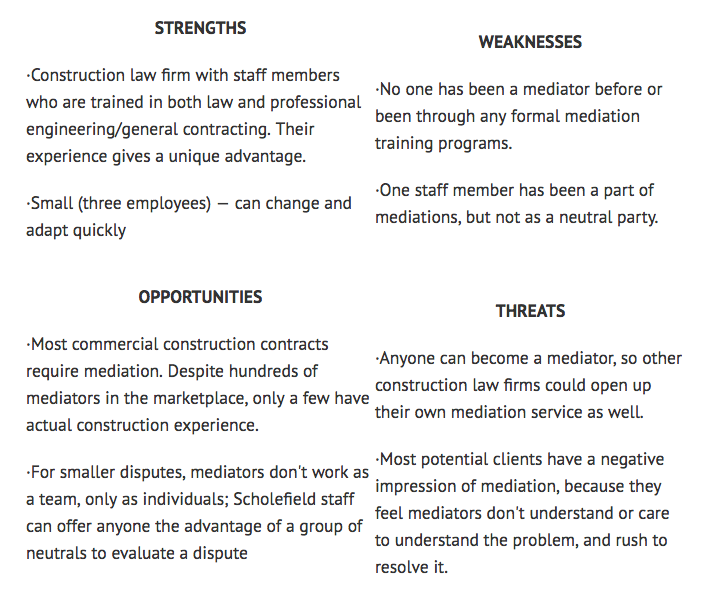
\includegraphics[width=\textwidth]{SWOTExample}
    \caption{Beispiel einer SWOT-Analyse. Quelle: http://www.businessnewsdaily.com/4245-swot-analysis.html}
    \label{fig:SWOTExample}          
\end{figure}

\subsubsection{PEST}
Bei der PEST-Analyse ist das Ziel, die politische, ökonomische, soziokulterelle und technologische Umfeld des Kunden zu verstehen. Dies ist eine reine Umfeld-Analyse und interne Punkte werden nicht aufgelistet. \\
\\
Da in den meisten Fällen bei der Analyse der Kunden für ein CSIRT sowohl interne wie auch externe Faktoren wichtig sind, bietet es sich an eine SWOT- und eine PEST-Analyse zu machen. So kann von Anfang an sichergestellt werden, dass nicht bereits bei der Planung des CSIRT in die falsche Richtung optimiert wird.

\subsection{Festlegen des Aufgabenbereichs}
Als nächstes muss der Aufgabenbereich des CSIRT definiert werden. Dies sollte eine möglichst kurz und knappe Formulierung sein, da diese der Grundstein des CSIRT ist und im besten Fall über Jahre hinweg Gültigkeit hat und nicht angepasst wird. Generell werden diese Formulierungen allgemein gehalten und enthalten keine spezifischen, prozessbedingten Angaben.

\subsection{Ausarbeitung des Geschäftsplans}
Nachdem der Aufgabenbereich definiert wurde, werden spezifischere Angaben im Geschäftsplan gemacht. 

\subsubsection{Finanzierung}
Oft ist in der Praxis die Finanzierung an ein bestimmtes Budget geknüpft. Die wichtigsten Faktoren sind die Dienstzeiten sowie die Anzahl Personenstellen, die für das CSIRT arbeiten.\\
\\
Dem gegenüber steht ein mögliches Ertragsmodell. Hierbei kommt es darauf an, an welche Kundenbedürfnisse sich das CSIRT richtet. Ist das CSIRT z.B. für die öffentliche Hand, sind Subventionen und Gelder vom Staat eine Option. Eine andere Option ist ein Mitgliedermodell mit Zusatzertrag gemäss Aufwand für Zusatzdienste z.B. Sicherheitsaudits.

\subsubsection{Organisation und Einstellen von Mitarbeitern}
Es gibt verschiedene Organisationsmodelle, die für ein CSIRT in Frage kommen. Entweder kann die CSIRT als eigenständige Organisation fungieren (d.h. mit eigener Geschäftsleitung etc.) oder kann als Team innerhalb einer bestehenden Organisation aufgebaut werden. Bei einer verteilten Organisation kann auch in Betracht gezogen werden, aus allen Standorten eine Person zu verpflichten. In der Praxis ist es schwierig, die genau erforderliche Anzahl Mitarbeiter zu bestimmen. Die ENISA spricht von mindestens vier Vollzeitstellen für das Verteilen von Security Advisories und Behandlung von Vorfällen. Übernimmt die CSIRT weitere Verantwortungen und muss z.B. Schichtdienst leisten, spricht die ENISA von mindestens 12 Vollzeitstellen. Hier gilt es die definierten Aufgabengebiete zu analysieren und die Kundenbedürfnisse korrekt zu analysieren. Eine Koordination mit anderen CSIRT kann von Vorteil sein, um z.B. eine 24/7 Abdeckung zu erhalten, bedingt aber das Lösen von anderen logistischen Herausforderungen.

\subsubsection{Richtlinien für die Informationssicherheit}
Je nach Kundentyp differenzieren die zu erstellenden Richtlinien zur Informationssicherheit. Es werden die betrieblichen sowie die administrativen Abläufe und Prozesse definiert. Wichtig dabei ist, dass nationale Richtlinien und Gesetze angewendet und befolgt werden. Viele Länder verfügen z.B. über Datenschutzgesetze, welche von allen eingehalten werden müssen. Ausserdem müssen Richtlinien definiert werden, die z.B. besagen wie Informationen klassifiziert und veröffentlicht werden. Grundsätzlich ist es zu empfehlen Security Advisories öffentlich zugänglich zu machen. Schwachstellen in Kunden-Systemen dürfen z.B. nicht vor dessen Behebung veröffentlicht werden. Eine genaue Spezifikation der Abläufe und Klassifikationen hilft dabei keine Kunden zu verärgern oder Gesetze zu missachten. Hier ist es auch wichtig die Geschäftsleitung mit einzubeziehen, damit organisationsweite Richtlinien mit eingebracht werden können. Natürlich sollte die Geschäftsleitung im gesamten Prozess mindestens ``informiert`` (siehe RASCI~\citep{rasci}) sein. In den meisten Fällen ergibt es jedoch Sinn, die Geschäftsleitung möglichst früh und eng einzubinden.

\section{Betrieb}
Nachfolgend werde ich einige Beispiele von Betriebsfällen nennen und erläutern, was dabei zu beachten ist.

\subsection{Analyse von Klienten}
Um für das Klientel die wichtige Aufgabe eines CSIRT auszuführen, ist es unabdingbar sich von der Umgebung der Klienten ein Bild zu machen. Dabei wird ein genaues Inventar geführt, welche Software bei welchen Kunden im Einsatz ist. Nur so kann effektiv informiert werden, falls eine Sicherheitslücke gefunden wird und entsprechend die Lage beurteilt werden. Wichtig dabei ist, dass diese auch aktuell gehalten wird, da ansonsten Warnungen gesendet werden, welche den Kunden gar nicht mehr betreffen. Dies dient zudem als Grundlage für alle weiteren Fälle.

\subsection{Alarme und Warnungen}
Anhand der oben erstellen Software-Liste können aktuelle und akute Sicherheits- und Bedrohungswarnungen an die Kunden gesendet werden. Hierbei gilt es zu beachten, dass nur Meldungen an Kunden gesendet werden, welche tatsächlich auch von dieser Vulnerability betroffen sind. Ansonsten führt das schnell zu einer ``Geht mich ja nichts an``-Wahrnehmung und die Kunden werden entsensibilisiert, was genau das Gegenteil des Zweckes einer CSIRT ist. Damit der Kunde die Bedrohung entsprechend einschätzen kann, ist es zu bevorziehen jeweils auch eine Analyse der Auswirkung des Incidents zu errechnen. Hierbei bedeutet die Auswirkung die Eintrittswahrscheinlichkeit multipliziert mit dem Risiko. \\
\\
Wichtig ist auch jeweils eine Empfehlung (z.B. Patch einspielen) für jedes Bulletin rauszugeben, damit die Kunden genau wissen, wie sie die Bedrohungslage verringern können. Zusätzlich ist es wichtig, dass diese Nachrichten durch den Kunden als vertrauenswürdig eingestuft werden können. Hierfür kann z.B. E-Mail-Signierung via GPG verwendet werden.

\subsection{Schulungen}
Ein weiterer, sehr wichtiger Punkt sind regelmässige Schulungen. Die IT-Landschaft und dessen Bedrohungen und Gefahren ändern sich fast täglich. Es ist wichtig, dass Angestellte immer auf dem aktuellsten Stand der Informationen sind, damit diese Kunden ihr Wissen entsprechend weitergeben können.\\
\\
Eine Sensibilisierung der Kunden ist genauso wichtig. Wenn ein Kunde zwar die Meldung erhält, dass es eine Bedrohung der IT-Sicherheit gibt, diese aber ignorieren, bzw. entgegen der Empfehlung als ``unwichtig`` einstufen, kann dies zu gravierenden Problemen führen. Daher ist es auch wichtig, Schulungen für Kunden zu veranstalten, um diese zu sensibilisieren.

\nomenclature[z-ENISA]{$ENISA$}{European Union Agency for Network and Information Security}
\nomenclature[z-swot]{$SWOT$}{Strengths, Weaknesses, Opportunities, Threats}
\nomenclature[z-pest]{$PEST$}{Political, Economical, Social, Technological}
\nomenclature[z-gpg]{$GPG$}{GNU Pretty Good Privacy}
\chapter{Erfolgsfaktoren eines CERT}

% **************************** Define Graphics Path **************************
\ifpdf
    \graphicspath{{Chapter3/Figs/Raster/}{Chapter3/Figs/PDF/}{Chapter3/Figs/}}
\else
    \graphicspath{{Chapter3/Figs/Vector/}{Chapter3/Figs/}}
\fi

\section{Aufbau - Kritische Erfolgsfaktoren}

\subsection{Einsatz von Ressourcen (Mitarbeiter, Zeit, Budget)}
Wie bei jedem Projekt muss sichergestellt werden, dass verfügbare Ressourcen korrekt und effektiv eingesetzt werden. Dabei sind sinnvolle Methodiken des Projektmanagementes anzuwenden. Mitarbeiter-Ressourcen, ihre verfügbare Zeit sowie auch das Budget sind hierbei die wichtigsten Faktoren. So muss z.B. sichergestellt werden, dass genügend Ressourcen vorhanden sind, jedoch ein Leerlauf möglichst verhindert wird. Hierbei gilt es jedoch darauf zu achten, dass der Einsatz von Ressourcen vernünftig ist. ``So wenig wie möglich`` ist hierbei der falsche Ansatz und führt zu mangelhafter Qualität.\\
\\
Im Vergleich zu anderen Erfolgsfaktoren sind diese mit gängigen Projektmanagement-Methoden messbar.

\subsection{Projektabschluss}
Analog zum Einsatz der Ressourcen ist bei Projekten auch der zeitlich vereinbarte Projektabschluss-Termin wichtig. Mit den angemessenen Projektplanungsmethoden kann die Wahrscheinlichkeit eines zu späten Abschlusses reduziert werden. Hierbei ist wichtig, dass mögliche Verspätungen schnellstmöglich kommuniziert werden, damit die Projektdauer entsprechend abgeschlossen werden kann. Verzögert sich der Abschluss des Projektes zu lange, besteht das Risiko, dass sich die Umgebung geändert hat und nicht mehr alle Bedürfnisse abgedeckt werden können. Eine zu grosse Fokussierung auf ``wir müssen das Projekt sofort abschliessen`` hindert jedoch die Umsetzung von qualitativ hochwertigen Ergebnissen.

\subsection{Unterstützung durch das Management}
Für beide oben genannten Erfolgsfaktoren ist es unabdingbar, dass das Management Unterstützung bietet. Es müssen Ressourcen geplant und Budget investiert werden. Schlussendlich sind dies Entscheidungen des Managements. Somit ist es wichtig, das Management frühzeitig und stetig in den Prozess des Aufbaus einzubinden und wo nötig zu konsultieren. In jedem Fall sollte das Management über den Projektstand regelmässig informiert werden. 

\subsection{Kundenglaubwürdigkeit}
Falls das Aufbau-Projekt von Kunden finanziert wird und nicht rein interner Natur ist, ist auch die Glaubwürdigkeit gegenüber der Kunden ein wichtiger Erfolgsfaktor. Der Kunde muss sicher sein, dass das aufzubauende Team in der Lage ist die gewünschten Dienstleistungen für die Kunden zu übernehmen. Hierbei ist z.B. wichtig, dass regelmässig über den Projektfortschritt kommuniziert wird, da auch im Betrieb des CSIRT schlussendlich Kommunikation einer der wichtigsten Bestandteile sein wird. Wird bereits während des Projektes nicht genügend kommuniziert, deutet dies auf eine Schwachstelle des Teams hin und es könnte davon ausgegangen werden, dass dies sich auch im Betrieb nicht ändern wird. Auch gegenüber Kunden, welche sich nicht finanziell am Projekt beteiligen, sollte regelmässig kommuniziert werden. Schlussendlich müssen die Kunden sicher sein, dass das Team ihre Anforderungen gewissenhaft, korrekt und zeitkritisch umsetzen kann.

\subsection{Bestehende Ressourcen / Hilfe von anderen CERTs}
Ein weiterer Erfolgsfaktor sind bestehende Ressourcen, bzw. Hilfe von anderen Teams. Soweit bestehende Ressourcen genutzt werden können, sollte auch darauf zugegriffen werden. Im CERT-Bereich sind viele Informationen öffentlich zugänglich. Diese sollten bereits beim Aufbau analysiert und eingebunden werden, da so das bestmögliche Ergebnis erreicht werden kann. \\
\\
Andere CERT können beim Aufbau wesentlich zur Qualität beitragen, da diese sich bereits im Betriebsstadium befinden und ggf. wichtige ``Lessions learned`` vermitteln können.

\section{Betrieb - Kritische Erfolgsfaktoren}

Beim Betrieb kommen fast die selben Kategorien von Erfolgsfaktoren zum Einsatz, da viele der Faktoren auch weiterhin gültig sind. 

\subsection{Einsatz von Ressourcen (Mitarbeiter, Zeit, Budget)}
Auch während des Betriebs muss sichergestellt werden, dass genügend Ressourcen vorhanden sind. Ein unterbesetztes CSIRT kann nicht die geforderten Leistungen erbringen und senkt somit die Kundenzufriedenheit. Wie in jeder anderen Organisation muss jedoch auch sichergestellt werden, dass die vorhandenen Ressourcen auch nach Projektabschluss vernünftig eingesetzt werden. 

\subsection{Unterstützung durch das Management}
Die Unterstützung des Managements ist weiterhin wichtig. Obwohl nach Projektabschluss ggf. ein Jahres-Budget vorhanden ist, muss wie bei jeder anderen Organisation auch, darauf geachtet werden, dass Änderungen der Managementstrategie in Einklang mit den Zielen des CSIRT gebracht werden. Ein kontinuierlicher Austausch zwischen Management und dem CSIRT-Team ist unabdingbar.

\subsection{Angebotene Dienstleistungen / Kundenzufriedenheit}
Erst während des Betriebs kann ermittelt werden, ob die angeboten Dienstleistungen den Kundenanforderungen entsprechen oder sich diese mittlerweile in eine andere Richtung bewegt haben. Die Kundenzufriendenheit betreffend Reaktionszeit, Qualität und Beratung kann z.B. mittels eines Fragebogens regelmässig überprüft werden. Zudem sollte regelmässig eine Analyse der Kunden (mit SWOT oder PEST) durchgeführt werden, um sicherzustellen, dass die angebotenen Dienstleistungen weiterhin die bestmögliche Qualität aufweisen. Dies ist einer der wichtigsten Faktoren für den Betrieb, da ohne Kunden (extern sowie auch intern) das Team nicht mehr benötigt wird und Dienstleistungen von anderen Anbietern angefordert werden.

\subsection{Dokumentation}
Um die Qualität und Zufriendeheit auf einem hohen Niveau zu halten, muss die Dokumentation immer wieder aktualisiert werden und allfällige ``Lessions learned`` angewendet werden. Nur so ist es möglich eine kontinuierlich hohe Qualität zu leisten und die Prozesse weiter zu verbessern. Die Dokumentation jedes Falles in einem ausreichenden Mass kann in Zukunft sehr wertvoll sein, auch wenn dies im ersten Augenblick nicht der Fall zu schein mag. Die Dokumentation hilft auch dabei neuen Mitarbeitern den Einstieg leichter zu machen und bereits vorhandenes Wissen zu vermitteln.

\subsection{Bestehende Ressourcen / Hilfe von anderen CERTs}
Während des Betriebs kann weiterhin auf die Mithilfe von anderen CERTs sowie auch auf den Zugriff von bestehenden Ressourcen gezählt werden. Je besser die Zusammenarbeit mit anderen Teams funktioniert, desto besser können die Kunden in ihren Anforderungen unterstützt und kompetent bedient werden.


%\include{Chapter4/chapter4}
%\include{Chapter5/chapter5}
%\include{Chapter6/chapter6}
%\include{Chapter7/chapter7}



% ********************************** Back Matter *******************************
% Backmatter should be commented out, if you are using appendices after References
%\backmatter

% ********************************** Bibliography ******************************
\begin{spacing}{0.9}

% To use the conventional natbib style referencing
% Bibliography style previews: http://nodonn.tipido.net/bibstyle.php
% Reference styles: http://sites.stat.psu.edu/~surajit/present/bib.htm

\bibliographystyle{apalike}
%\bibliographystyle{unsrt} % Use for unsorted references  
%\bibliographystyle{plainnat} % use this to have URLs listed in References
\cleardoublepage
\bibliography{References/references} % Path to your References.bib file


% If you would like to use BibLaTeX for your references, pass `custombib' as
% an option in the document class. The location of 'reference.bib' should be
% specified in the preamble.tex file in the custombib section.
% Comment out the lines related to natbib above and uncomment the following line.

%\printbibliography[heading=bibintoc, title={References}]


\end{spacing}

% ********************************** Appendices ********************************

%\begin{appendices} % Using appendices environment for more functunality

%\include{Appendix1/appendix1}
%\include{Appendix2/appendix2}

%\end{appendices}

% *************************************** Index ********************************
%\printthesisindex % If index is present

\end{document}